\chapter{Methodology}

\vspace{-1cm}

This chapter shows the process of designing, testing and troubleshooting tools and equipment, construction and wiring procedure.

Now that the design is in place, the purchase of material will follow, then the construction of the device and lastly the performance, 
functionality, and reliability will be tested.

\section{System Design}
\begin{figure}[ht]
\centering \begin{tikzpicture}
  \node[anchor=north west] (battery) at (0, -0.3) {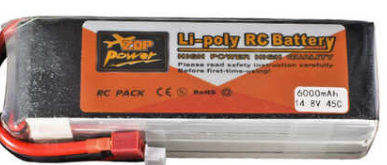
\includegraphics[width=3cm]{assets/battery.png}};
  \node[anchor=north west] (converter) at (5, 0) {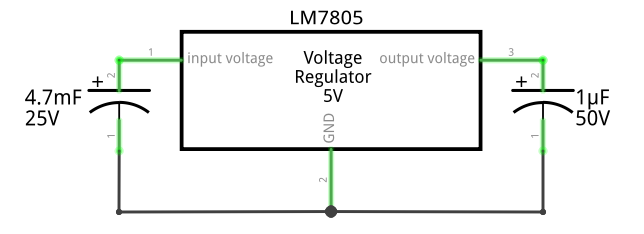
\includegraphics[width=5cm]{assets/converter.png}};
  \node[anchor=north west] (esp32) at (6, -3.5) {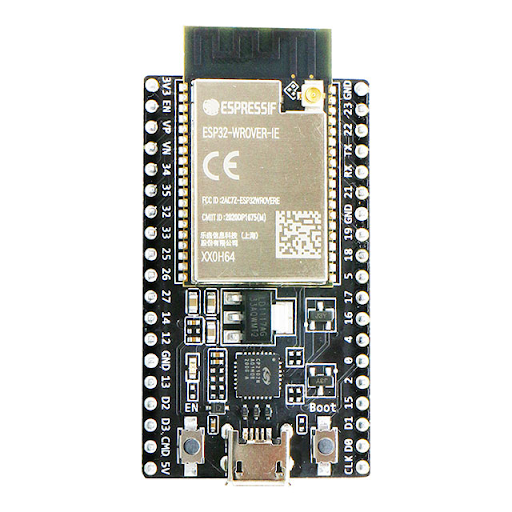
\includegraphics[width=3cm]{assets/esp-32.png}};
  \node[anchor=north west] (magnetometer) at (12, -1) {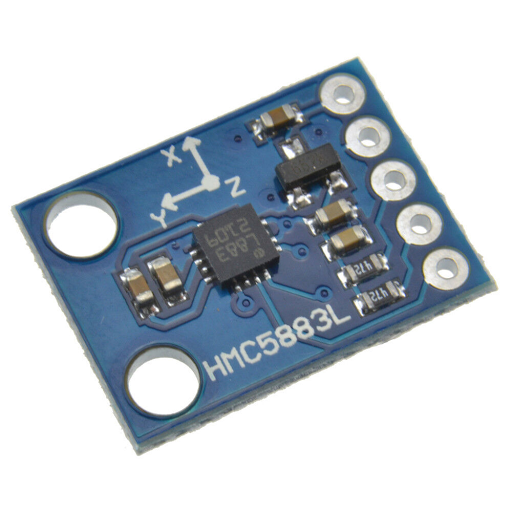
\includegraphics[width=3cm]{assets/magnetometer.png}};
  \node[anchor=north west] (gps) at (12, -5.5) {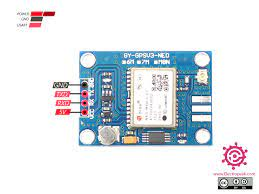
\includegraphics[width=3cm]{assets/gps_module.png}};
  \node[anchor=north west] (esc) at (0, -3.5) {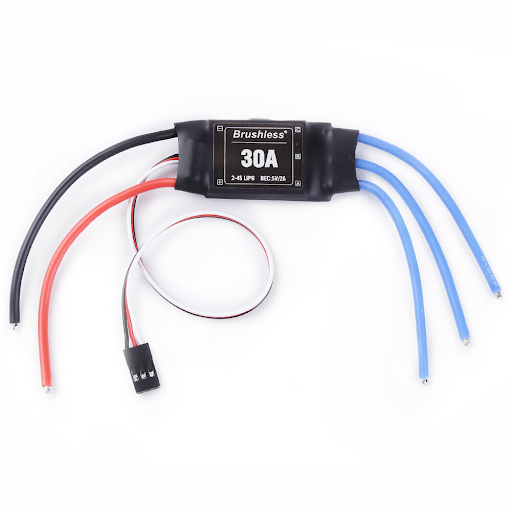
\includegraphics[width=3cm]{assets/esc.png}};
  \node[anchor=north west] (motor) at (3, -8) {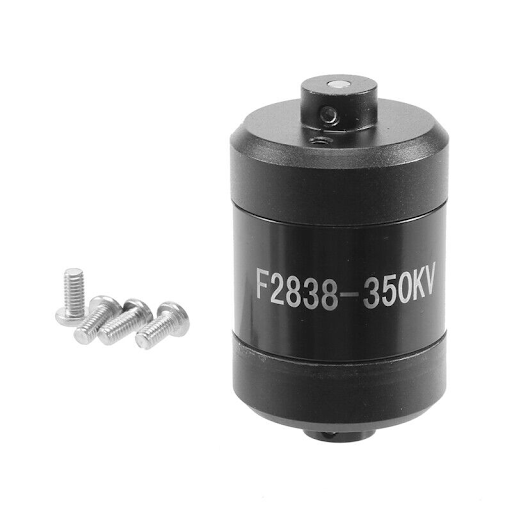
\includegraphics[width=3cm]{assets/motor.png}};
  \node[anchor=north west] (propeller) at (9, -8.2) {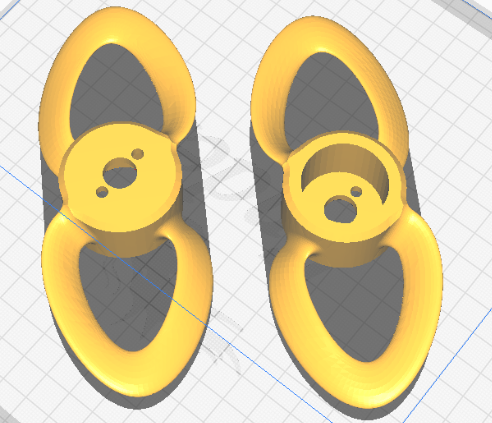
\includegraphics[width=3cm]{assets/propellers.png}};

  \draw[ ->, line width = 1mm, black!70] (battery) to node[] {} (converter);
  \draw[ ->, line width = 1mm, black!70] (battery) to node[] {} (esc);
  \draw[ ->, line width = 1mm, black!70] (esp32) to node[] {} (esc);
  \draw[ ->, line width = 1mm, black!70] (esc) to node[] {} (motor);
  \draw[ ->, line width = 1mm, black!70] (motor) to node[] {} (propeller);
  \draw[ ->, line width = 1mm, black!70] (converter) to node[] {} (esp32);
  \draw[ <->, line width = 1mm, black!70] (esp32) to node[] {} (magnetometer);
  \draw[ <->, line width = 1mm, black!70] (esp32) to node[] {} (gps);

\end{tikzpicture}
\caption{System Design}
\label{fig:SystemDesign}
\end{figure}

\pagebreak

\section{Flowchart}
\begin{figure}[ht]
\centering \begin{tikzpicture}
  [
  RECT/.style={rectangle, rounded corners, draw=black!60, fill=white!0, very thick, minimum width = 20mm, minimum height = 10mm, align = center},
  ROUNDEDRECT/.style={rounded rectangle, draw=black!60, fill=white!0, very thick, minimum width = 20mm, minimum height = 10mm},
  DIAMOND/.style={diamond, draw=black!60, fill=white!0, very thick, minimum width = 10mm, minimum height = 10mm, align = center, aspect = 2, },
  ]

  \node[ROUNDEDRECT] (start) {Start};
  \node[RECT] (switchOn) [below = of start] {Switch on};
  \node[RECT] (esp32Boot) [right = of switchOn] {ESP-32 boots};
  \node[RECT] (waitForUserInput) [right = of esp32Boot] {Waiting for user \\ input coordinates};
  \node[RECT] (coordinatesSupplied) [below = of waitForUserInput] {Coordinates Supplied};
  \node[RECT] (detectsLocationData) [left = of coordinatesSupplied] {GPS \& magnetometer \\ detects location data};
  \node[RECT] (droneMoves) [left = of detectsLocationData] {Drone moves to \\ supplied coordinates};
  \node[RECT] (confirmLoc) [below = of droneMoves] {GPS \& magnetometer \\ confirms location data};
  \node[] (dummyNode) [below = of detectsLocationData] {};
  \node[DIAMOND] (doesLocMatch) [below = of dummyNode] {Does drone location match \\ with supplied coordinates?};
  \node[RECT] (terminate) [below = of doesLocMatch] {Drone terminated};
  \node[ROUNDEDRECT] (end) [right = of terminate] {End};

  \draw[ ->, line width = 1mm, black!70] (start.south) to node[] {} (switchOn.north);
  \draw[ ->, line width = 1mm, black!70] (switchOn.east) to node[] {} (esp32Boot.west);
  \draw[ ->, line width = 1mm, black!70] (esp32Boot.east) to node[] {} (waitForUserInput.west);
  \draw[ ->, line width = 1mm, black!70] (waitForUserInput.south) to node[] {} (coordinatesSupplied.north);
  \draw[ ->, line width = 1mm, black!70] (coordinatesSupplied.west) to node[] {} (detectsLocationData.east);
  \draw[ ->, line width = 1mm, black!70] (detectsLocationData.west) to node[] {} (droneMoves.east);
  \draw[ ->, line width = 1mm, black!70] (droneMoves.south) to node[] {} (confirmLoc.north);
  \draw[ ->, line width = 1mm, black!70] (confirmLoc.south) to node[] {} (doesLocMatch.west);
  \draw[ ->, line width = 1mm, black!70] (doesLocMatch.north) to node[left] {NO} (detectsLocationData.south);
  \draw[ ->, line width = 1mm, black!70] (doesLocMatch.south) to node[left] {YES} (terminate.north);
  \draw[ ->, line width = 1mm, black!70] (terminate.east) to node[] {} (end.west);
\end{tikzpicture}
\caption{Flowchart}
\label{fig:Flowchart}
\end{figure}